% Generated by eval/scripts/write_reference_comparison_figures.py.
\definecolor{srweak}{RGB}{35,103,159}
\definecolor{srstrong}{RGB}{202,86,42}
\definecolor{belebeleif}{RGB}{35,103,159}
\definecolor{belebelecons}{RGB}{202,86,42}
\definecolor{belebelespec}{RGB}{38,132,109}
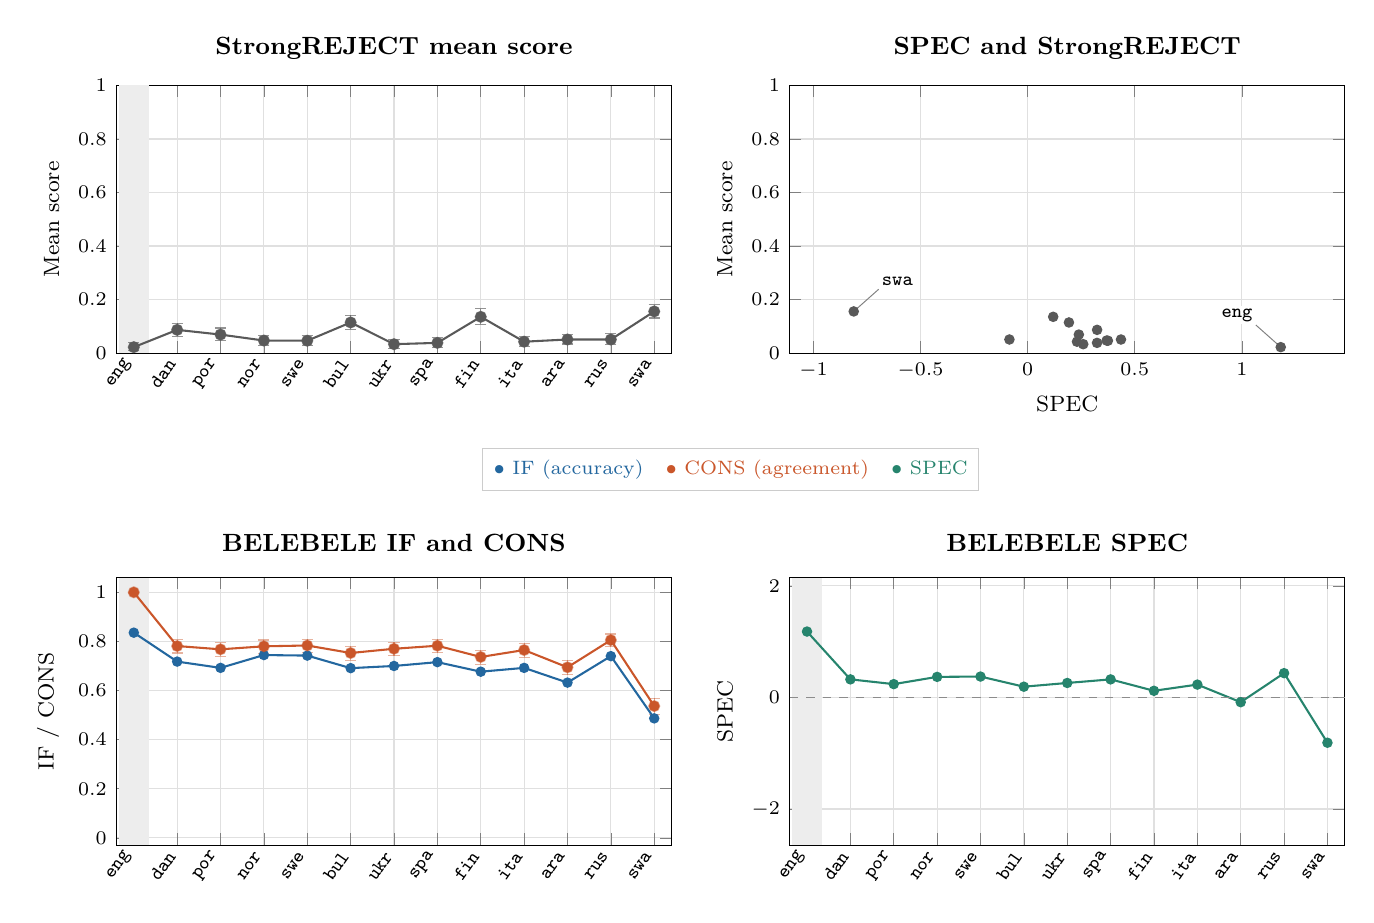
\begin{tikzpicture}
\pgfplotsset{srprofile/.style={width=7.05cm,height=2.65cm,scale only axis,xmin=-.4,xmax=12.4,ymin=0,ymax=1,ytick={0,.2,.4,.6,.8,1},axis lines=box,grid=major,grid style={black!12},tick label style={font=\scriptsize},label style={font=\footnotesize},title style={font=\bfseries\small},xtick={0,...,12},x tick label style={rotate=55,anchor=east,font=\scriptsize},ylabel={Mean score}}}
\pgfplotsset{srscatter/.style={width=7.05cm,height=2.65cm,scale only axis,ymin=0,ymax=1,ytick={0,.2,.4,.6,.8,1},xlabel={SPEC},ylabel={Mean score},axis lines=box,grid=major,grid style={black!12},tick label style={font=\scriptsize},label style={font=\footnotesize},title style={font=\bfseries\small},enlarge x limits=.15}}
\pgfplotsset{belebeleaxis/.style={width=7.05cm,scale only axis,xmin=-.4,xmax=12.4,
axis lines=box,grid=major,grid style={black!12},
tick label style={font=\scriptsize},label style={font=\footnotesize},
title style={font=\bfseries\small},unbounded coords=jump,
clip=true,xtick={0,...,12}}}
\begin{axis}[srprofile,height=3.4cm,at={(0cm,0cm)},anchor=north west,title={StrongREJECT mean score},xticklabels={\texttt{\textbf{eng}},\texttt{dan},\texttt{por},\texttt{nor},\texttt{swe},\texttt{bul},\texttt{ukr},\texttt{spa},\texttt{fin},\texttt{ita},\texttt{ara},\texttt{rus},\texttt{swa}}]
\path[fill=black!7] (axis cs:-.35,0) rectangle (axis cs:.35,1);
\addplot[color=black!65,mark=*,mark size=1.6pt,line width=.75pt] coordinates {(0,0.022364) (1,0.086939) (2,0.069311) (3,0.047026) (4,0.046371) (5,0.114550) (6,0.033416) (7,0.038339) (8,0.135666) (9,0.042732) (10,0.050971) (11,0.050881) (12,0.155744)};
\addplot[color=black!65,opacity=.65,only marks,mark=none,error bars/.cd,y dir=both,y explicit] coordinates {(0,0.022364) += (0,0.017572) -= (0,0.013978) (1,0.086939) += (0,0.025250) -= (0,0.024439) (2,0.069311) += (0,0.024439) -= (0,0.022837) (3,0.047026) += (0,0.020096) -= (0,0.017685) (4,0.046371) += (0,0.020575) -= (0,0.018558) (5,0.114550) += (0,0.026929) -= (0,0.025332) (6,0.033416) += (0,0.017337) -= (0,0.014851) (7,0.038339) += (0,0.018770) -= (0,0.016783) (8,0.135666) += (0,0.030717) -= (0,0.027730) (9,0.042732) += (0,0.019569) -= (0,0.018371) (10,0.050971) += (0,0.017799) -= (0,0.016990) (11,0.050881) += (0,0.021635) -= (0,0.018440) (12,0.155744) += (0,0.024676) -= (0,0.024676)};
\end{axis}
\begin{axis}[srscatter,height=3.4cm,at={(8.55cm,0cm)},anchor=north west,title={SPEC and StrongREJECT}]
\addplot[only marks,color=black!65,mark=*,mark size=1.7pt] coordinates {(1.181697,0.022364) (0.324334,0.086939) (0.239115,0.069311) (0.368920,0.047026) (0.374768,0.046371) (0.192872,0.114550) (0.259633,0.033416) (0.324048,0.038339) (0.119382,0.135666) (0.230438,0.042732) (-0.084995,0.050971) (0.435809,0.050881) (-0.811875,0.155744)};
\node[font=\scriptsize,anchor=south east,xshift=-9pt,yshift=8pt,fill=white,inner sep=1pt] (languageLabel0) at (axis cs:1.181697,0.022364) {\texttt{eng}};
\draw[black!50,line width=.35pt] (languageLabel0.south east) -- (axis cs:1.181697,0.022364);
\node[font=\scriptsize,anchor=south west,xshift=9pt,yshift=8pt,fill=white,inner sep=1pt] (languageLabel1) at (axis cs:-0.811875,0.155744) {\texttt{swa}};
\draw[black!50,line width=.35pt] (languageLabel1.south west) -- (axis cs:-0.811875,0.155744);
\end{axis}
\node[anchor=south,draw=black!20,fill=white,inner sep=4pt,font=\scriptsize] at (7.8,-5.15) {\textcolor{belebeleif}{$\bullet$ IF (accuracy)}\quad
\textcolor{belebelecons}{$\bullet$ CONS (agreement)}\quad
\textcolor{belebelespec}{$\bullet$ SPEC}};
\begin{axis}[belebeleaxis,height=3.4cm,at={(0.0cm,-6.25cm)},anchor=north west,ymin=-.03,ymax=1.06,ytick={0,.2,.4,.6,.8,1},ylabel={IF / CONS},title={BELEBELE IF and CONS},xticklabels={\texttt{\textbf{eng}},\texttt{dan},\texttt{por},\texttt{nor},\texttt{swe},\texttt{bul},\texttt{ukr},\texttt{spa},\texttt{fin},\texttt{ita},\texttt{ara},\texttt{rus},\texttt{swa}},x tick label style={rotate=55,anchor=east,font=\scriptsize}]
\path[fill=black!7] (axis cs:-.35,-.03) rectangle (axis cs:.35,1.06);
\addplot[color=belebeleif,mark=*,mark size=1.5pt,line width=.75pt] coordinates {(0,0.835556) (1,0.717778) (2,0.692222) (3,0.744444) (4,0.742222) (5,0.691111) (6,0.700000) (7,0.715556) (8,0.676667) (9,0.692222) (10,0.632222) (11,0.740000) (12,0.486667)};
\addplot[color=belebelecons,mark=*,mark size=1.5pt,line width=.75pt] coordinates {(0,1.000000) (1,0.781111) (2,0.767778) (3,0.780000) (4,0.783333) (5,0.752784) (6,0.770000) (7,0.782366) (8,0.736667) (9,0.764838) (10,0.694444) (11,0.805369) (12,0.536667)};
\addplot[color=belebelecons,opacity=.45,only marks,mark=none,error bars/.cd,y dir=both,y explicit] coordinates {(0,1.000000) += (0,0.000000) -= (0,0.004250) (1,0.781111) += (0,0.025789) -= (0,0.028178) (2,0.767778) += (0,0.026413) -= (0,0.028689) (3,0.780000) += (0,0.025842) -= (0,0.028222) (4,0.783333) += (0,0.025681) -= (0,0.028089) (5,0.752784) += (0,0.027099) -= (0,0.029252) (6,0.770000) += (0,0.026312) -= (0,0.028607) (7,0.782366) += (0,0.025782) -= (0,0.028193) (8,0.736667) += (0,0.027726) -= (0,0.029737) (9,0.764838) += (0,0.026645) -= (0,0.028914) (10,0.694444) += (0,0.029216) -= (0,0.030869) (11,0.805369) += (0,0.024624) -= (0,0.027237) (12,0.536667) += (0,0.032353) -= (0,0.032665)};
\end{axis}
\begin{axis}[belebeleaxis,height=3.4cm,at={(8.55cm,-6.25cm)},anchor=north west,ymin=-2.65,ymax=2.15,ytick={-2,0,2},ylabel={SPEC},title={BELEBELE SPEC},xticklabels={\texttt{\textbf{eng}},\texttt{dan},\texttt{por},\texttt{nor},\texttt{swe},\texttt{bul},\texttt{ukr},\texttt{spa},\texttt{fin},\texttt{ita},\texttt{ara},\texttt{rus},\texttt{swa}},x tick label style={rotate=55,anchor=east,font=\scriptsize}]
\path[fill=black!7] (axis cs:-.35,-2.65) rectangle (axis cs:.35,2.15);
\addplot[color=belebelespec,mark=*,mark size=1.5pt,line width=.75pt] coordinates {(0,1.181697) (1,0.324334) (2,0.239115) (3,0.368920) (4,0.374768) (5,0.192872) (6,0.259633) (7,0.324048) (8,0.119382) (9,0.230438) (10,-0.084995) (11,0.435809) (12,-0.811875)};
\addplot[black!45,dashed,mark=none] coordinates {(-.4,0) (12.4,0)};
\end{axis}
\end{tikzpicture}
